\documentclass[12pt, twoside]{article}
\usepackage[letterpaper, margin=1in, headsep=0.5in]{geometry}
\usepackage[english]{babel}
\usepackage[utf8]{inputenc}
\usepackage{amsmath}
\usepackage{amsfonts}
\usepackage{amssymb}
\usepackage{tikz}
\usetikzlibrary{quotes, angles}
\usepackage{graphicx}
\usepackage{enumitem}
\usepackage{multicol}
\usepackage{hyperref}

\newif\ifmeta
\metatrue %print standards and topics tags

\title{IB Mathematics}
\author{Chris Huson}
\date{January 2022}

\usepackage{fancyhdr}
\pagestyle{fancy}
\fancyhf{}
\renewcommand{\headrulewidth}{0pt} % disable the underline of the header
\raggedbottom


\fancyhead[LE]{\thepage}
\fancyhead[RO]{\thepage \\ Name: \hspace{4cm} \,\\}
\fancyhead[LO]{BECA / PreCalculus / SAT Prep \\* 13 February 2023}

\begin{document}

\subsubsection*{9.1 Classwork: Linear and quadratic graphs}
\begin{enumerate}
\item A linear function $f$ is graphed below.
    \begin{multicols}{2}
    \begin{enumerate}
      \item Write down it's slope.\\ $m=$
      \vspace{0.25cm}
      \item Write down it's $y$-intercept.\\ $b=$
      \vspace{0.25cm}
      \item Write down the equation of the line.
      \vspace{1cm}
      \item State the coordinates of the point $Q$.
    \end{enumerate} \vspace{.5cm}
      \begin{center} 
      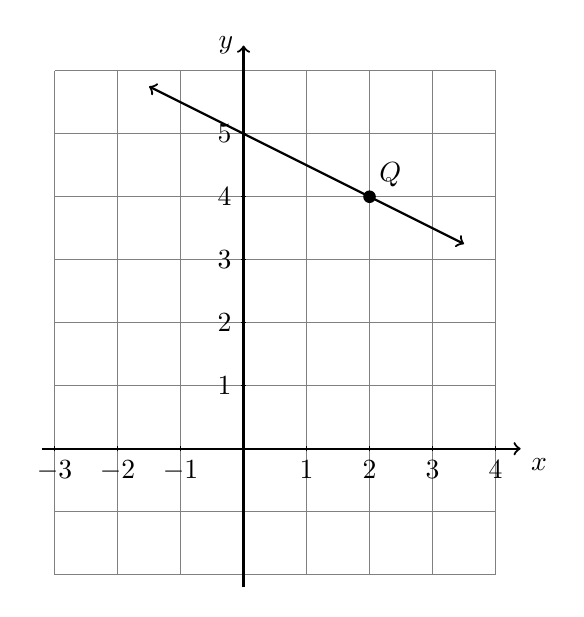
\begin{tikzpicture}[scale=0.8]
        \draw [help lines] (-3,-2) grid (4,6);
        \draw [thick, ->] (-3.2,0) -- (4.4,0) node [below right] {$x$};
        \draw [thick, ->] (0,-2.2)--(0,6.4) node [left] {$y$};
        \foreach \x in {-3,-2,-1,1,2,...,4} \draw (\x cm,1pt) -- (\x cm,-1pt) node[anchor=north] {$\x$};
        \foreach \y in {1, 2, 3, 4, 5} \draw (1pt,\y cm) -- (-1pt,\y cm) node[anchor=east] {$\y$};
        \draw [thick, <->,smooth,samples=20,domain=-1.5:3.5] plot(\x,-0.5*\x+5);
        \fill (2,4) circle[radius=0.1] node[above right]{$Q$};
      \end{tikzpicture}
      \end{center}
    \end{multicols}
    
\item Write the linear equation $\displaystyle y-1=\frac{1}{2}(x+8)$ in the form $y=mx+c$. \vspace{4cm}

\item Given $f(x)=(x-1)(x+5)$
    \begin{enumerate}[itemsep=0.9cm]
        \begin{multicols}{2}
        \item Sketch the function. Label the vertex as an ordered pair and mark the intercepts with their values.
        \item Expand the function to standard form, $f(x)=ax^2+bx+c \text{ where } a, b, c \;  \epsilon \; \mathbb{R}$. \vspace{3.5cm}
        \begin{center}
            \begin{tikzpicture}
                \draw [thick, ->] (-3.5,0) -- (+3.5,0) node [below left] {$x$};
                \draw [thick, ->] (0,-4.5) -- (0,3) node [left] {$y$};
            \end{tikzpicture}
            \end{center}
        \end{multicols}
    \end{enumerate}

\item The function $f(x)=-\frac{1}{2}x^{2}+2x$ is shown on the graph.
    \begin{enumerate}[itemsep=1.2cm]
      \begin{multicols}{2}
          \item Write down its vertex as an ordered pair.
          \item Write down its domain and range.
          \item Write down $f(0)$.
          \item Write down two solutions to $f(x)=0$. 
          %\item Hence or otherwise, write $f$ in the form $f(x)=a(x-p)(x-q)$\vspace{3cm}
          \begin{center}
          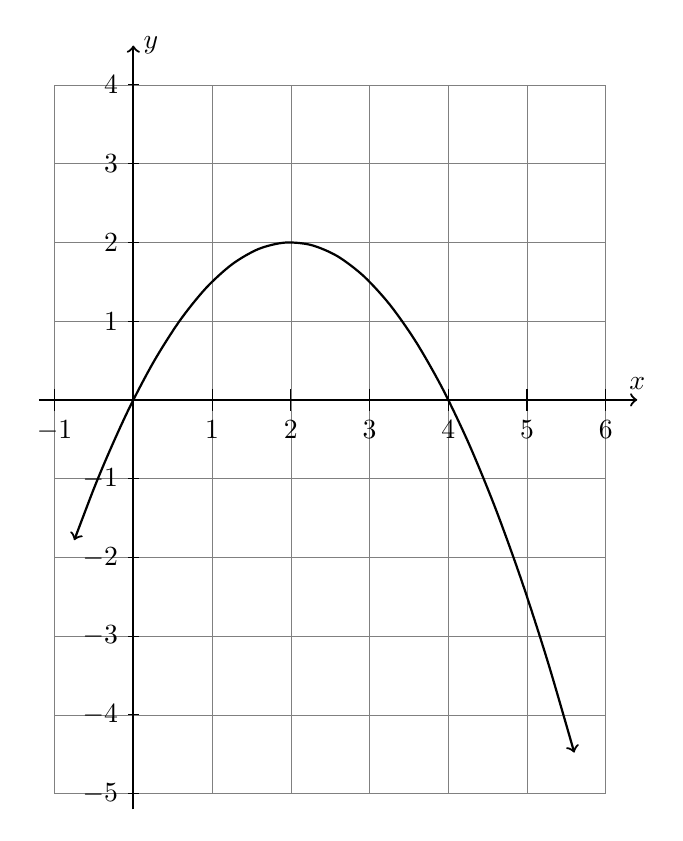
\begin{tikzpicture}[scale=1]
            \draw [help lines] (-1,-5) grid (6,4);
            \draw [thick, ->] (-1.2,0) -- (6.4,0) node [above] {$x$};
            \draw [thick, ->] (0,-5.2)--(0,4.5) node [right] {$y$};
            \foreach \x in {-1, 1,2, ...,6} \draw (\x cm,4pt) -- (\x cm,-4pt) node[below] {$\x$};
            \foreach \y in {-5,...,-1,1,2,...,4} \draw (2pt,\y cm) -- (-2pt,\y cm) node[left] {$\y$};
            %\fill (-1,0) circle[radius=0.1] node[above left]{$j$};
            %\fill (3,0) circle[radius=0.1] node[above right]{$k$};
            \draw [thick, <->,smooth,samples=20,domain=-0.75:5.6] plot(\x,-0.5*\x*\x+2*\x);
          \end{tikzpicture}
          \end{center}
        \end{multicols}
    \end{enumerate} \vspace{2cm}
    
\item Consider the function $f(x)=x^2+4x-12$. (graph it to answer the questions)
\begin{enumerate}
    %\item Sketch the graph of $f$, for $-4 \leq x \leq 2$. Label the vertex and the intercepts.
    \item This function can also be written in the form $f(x)=(x-p)^2 -16$.\\* 
    Write down the value of $p$. \vspace{1.5cm}
    \item The graph of $f$ has two solutions for $f(x)=0$. Write down the solutions (or roots, zeros) of the function. \vspace{1.5cm}
    \item Hence, write down the function in factored form, $f(x)=(x-a)(x-b)$. \vspace{1.5cm}
\end{enumerate}
    
\newpage
\item Given two functions, a quadratic function $f(x)=0.8x^2+3.2x-2$ and a linear function $g(x)=0.8x+1.2$.
    \begin{enumerate}%[itemsep=1cm]
        \item Graph the parabola $y=f(x)$, marking the $y$-intercept and the vertex as an ordered pair.
        \item Find the coordinates of the two intercepts with the $x$-axis, the roots or zeros of $f(x)$.\vspace{1cm}
        \item Plot the linear function, $y=g(x)$. Mark and label the two intersections of the two functions $f(x)=g(x)$ as ordered pairs.
    \end{enumerate}
    \begin{center}
    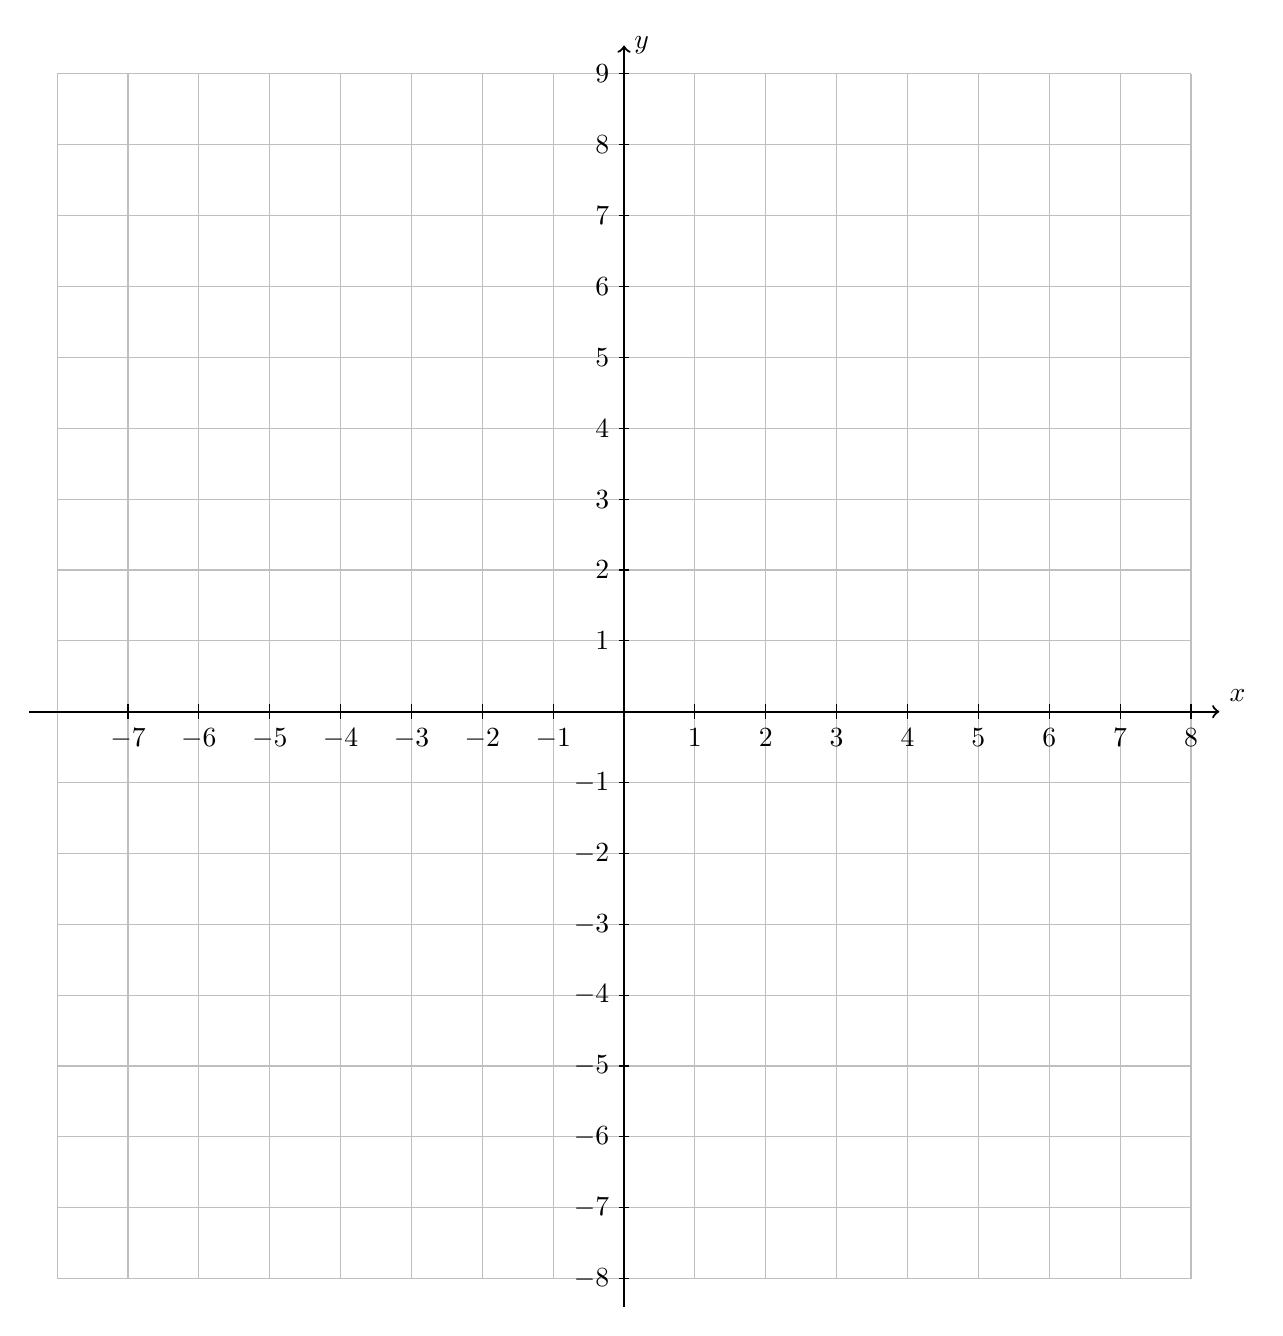
\begin{tikzpicture}[scale=0.9]
        \draw [thin, color=lightgray,, xstep=1.0cm,ystep=1.0cm] (-8,-8) grid (8,9);
        \foreach \x in {-7,...,-1,1,2,...,8}
        \draw (\x cm,3pt) -- (\x cm,-3pt) node[below] {$\x$};
        \foreach \y in {-8,...,-1,1,2,...,9}
        \draw[shift={(0,\y)},color=black] (2pt,0pt) -- (-2pt,0pt) node[left]  {$\y$};
        \draw [thick, ->] (-8.4,0) -- (+8.4,0) node [above right] {$x$};
        \draw [thick, ->] (0,-8.4) -- (0,9.4) node [right] {$y$};
        %\draw [thick, <->,smooth,domain=-5:2] plot(\x,0.8*\x*\x+3.2*\x-2);
    \end{tikzpicture}
    \end{center}

\newpage


\newpage
\item A dart is shot vertically upwards.\\[0.25cm]
The path of the dart can be modelled by the equation $h(t)=8t-t^2$ where $h(t)$ is the height in meters of the dart after $t$ seconds.
    \begin{enumerate}
        \item Plot a graph of this equation and hence sketch it below, showing the coordinates of the vertex and axes intercepts.
        \item Find the $t$-intercepts and explain what these values represent. \vspace{2cm}
        \item Find the equation of the axis of symmetry, and state what this tells you in the context of the problem. \vspace{2cm}
    \end{enumerate}
    \begin{center}
    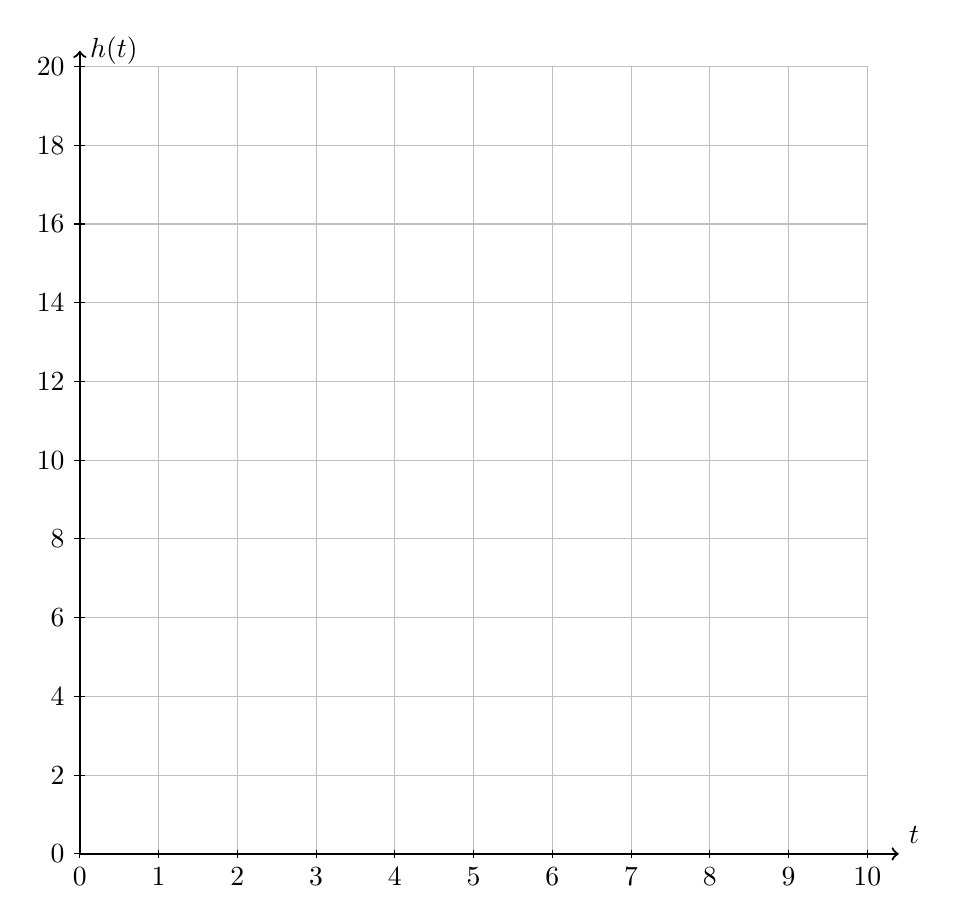
\begin{tikzpicture}[yscale=0.5]
        \draw [thin, color=lightgray,, xstep=1.0cm,ystep=2.0cm] (0,0) grid (10,20);
        \foreach \x in {0,1,2,...,10}
        \draw (\x cm,3pt) -- (\x cm,-3pt) node[below] {$\x$};
        \foreach \y in {0,2,...,20}
        \draw[shift={(0,\y)},color=black] (2pt,0pt) -- (-2pt,0pt) node[left]  {$\y$};
        \draw [thick, ->] (0,0) -- (+10.4,0) node [above right] {$t$};
        \draw [thick, ->] (0,0) -- (0,20.4) node [right] {$h(t)$};
        %\draw [thick, <->,smooth,domain=-0.5:8.5] plot(\x,-\x*\x+8*\x);
    \end{tikzpicture}
    \end{center}

\end{enumerate}
\end{document}